\def\probtitle{Traveling SCCC President}
\def\probno{G}

\begin{problem}{\probno{}. \probtitle{}}

숭실대학교 컴퓨터학부 문제해결 소모임 SCCC의 회장인 찬솔이는 대회를 성공적으로 개최하기 위해 학교의 여러 건물에 들려 업무를 보고 있다.

숭실대학교의 캠퍼스는 $1$번부터 $N$번까지 번호가 붙어 있는 $N$개의 건물과 서로 다른 두 건물을 연결하고 $1$번부터 $M$번까지 번호가 붙어 있는 $M$개의 도로로 구성되어 있다. $i$번 도로는 $u_i$번 건물과 $v_i$번 건물을 연결하고, 이 도로를 이용해 한 쪽 건물에서 다른 쪽 건물로 이동하는데 $w_i$분이 걸린다. 모든 건물은 도로를 통해 이어져 있다.

대회를 개최하기 위해서는 $N$개의 건물에서 한 번씩 \textbf{차례대로} 회의를 진행해야 한다. 구체적으로, 회의를 진행해야 하는 건물의 순서 $A_1, A_2, \cdots, A_N$이 주어진다. $i$번째로 진행해야 하는 회의는 $A_i$번 건물에서 진행되며, 모든 $A_i$는 서로 다르다.

4차 산업혁명이 도래한 21세기에 매번 도로를 통해 이동하는 것은 비효율적이기 때문에, 찬솔이는 순간 이동 장치를 만들었다. 순간 이동 장치를 사용하면 지금까지 방문했던 건물 중 원하는 곳으로 순식간에 이동할 수 있다.

찬솔이는 $S$번 건물에서 출발해서 $N$개의 회의를 마친 다음 다시 $S$번 건물로 돌아와야 한다. 시간이 부족한 찬솔이를 위해 $N$개의 회의를 차례대로 모두 마치고 $S$번 건물로 돌아오는데 걸리는 최소 시간을 구해주자.

예를 들어 숭실대학교 캠퍼스가 아래 그림과 같은 형태이고 $1$번 건물에서 출발하며, $1, 3, 2$번 건물에서 차례대로 회의를 진행해야 한다고 하자.

\begin{center}
    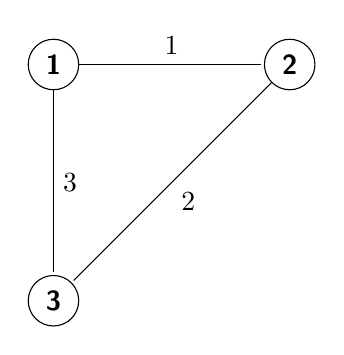
\begin{tikzpicture}[shorten >=1pt, auto, node distance=3cm]
        \begin{scope}[every node/.style={circle,draw=black,font=\sffamily\bfseries}]
            \node (1) at (-1.5, 1.5) {1};
            \node (2) at (1.5, 1.5) {2};
            \node (3) at (-1.5, -1.5) {3};
        \end{scope}
        \begin{scope}[every edge/.style={draw=black}]
            \draw (1) edge node{1} (2);
            \draw (1) edge node{3} (3);
            \draw (2) edge node{2} (3);
        \end{scope}
    \end{tikzpicture}
\end{center}

% \textbf{\textcolor{red}{@TODO 그림 추가}}

찬솔이는 먼저 1번 건물에서 회의를 진행한 뒤, 도로를 통해 2번 건물을 거쳐 3번 건물로 이동해서 회의를 진행한다. 이후 순간 이동 장치를 사용해 2번 건물로 이동해 회의를 진행한 뒤, 순간 이동 장치를 써서 1번 건물로 돌아올 수 있다. 이 과정에서 소요되는 총 시간은 3분이다.

\InputFile

첫째 줄에 건물의 개수 $N$, 도로의 개수 $M$, 출발하는 건물의 번호 $S$가 공백으로 구분되어 주어진다.

둘째 줄부터 $M$개의 줄에 걸쳐, $i$번 도로가 연결하는 두 건물의 번호 $u_i, v_i$와 도로를 통행하는 데 걸리는 시간 $w_i$가 한 줄에 하나씩 공백으로 구분되어 주어진다.

$M+2$번째 줄에는 $N$개의 정수 $A_1, A_2, \cdots, A_N$이 주어진다. 이는 $i$번째 회의가 $A_i$번 건물에서 진행됨을 의미한다.

\newpage

\OutputFile

$S$번 건물에서 출발해서 $N$개의 회의를 \textbf{차례대로} 마친 다음에 다시 $S$번 건물로 돌아오는 데 필요한 최소 시간을 출력한다.

\Constraints

\begin{itemize}[noitemsep]
    \item $2 \leq N \leq 2\,000$
    \item $N-1 \leq M \leq 5\,000$
    \item $1 \leq S \leq N$
    \item $1 \leq u_i < v_i \leq N$ $(1 \le i \le M)$
    \item $1 \leq w_i \leq 5\,000$ $(1 \le i \le M)$
    \item $A$에는 $1$부터 $N$까지의 정수가 정확히 한 번씩 등장한다.
    \item 모든 건물은 도로를 통해 이어져 있다.
    \item 입력으로 주어지는 수는 모두 정수이다.
\end{itemize}

\Example

\begin{example}
    \exmpfile{./example/01.in.txt}{./example/01.out.txt}%
    \exmpfile{./example/02.in.txt}{./example/02.out.txt}%
\end{example}

% \newpage

% \Notes


\end{problem}